\documentclass[11pt,a4paper]{article}
\usepackage[utf8]{inputenc}
\usepackage[english]{babel}
\usepackage[T1]{fontenc}
\usepackage{charter}
\usepackage{amsmath}
\usepackage{amsfonts}
\usepackage{amssymb}
\usepackage{esint}
\usepackage[table]{xcolor}
\usepackage{graphicx}
\usepackage[left=1.5cm,right=1.5cm,top=2cm,bottom=2cm]{geometry}
\usepackage{tikz}
\usepackage{tikz-3dplot}
\usetikzlibrary{babel}
\usepackage[font=small,labelfont={small,bf},margin=0.5cm,justification=justified]{caption}
\usepackage[font=small,labelfont={small,bf}]{subcaption}
\usepackage{epstopdf}
\usepackage{natbib}
\usepackage[nointegrals]{wasysym}
%\renewcommand\familydefault\sfdefault
\usepackage[italic,defaultmathsizes]{mathastext}
\usepackage{hyperref}
\usepackage{lipsum}
\usepackage{threeparttable}
\usepackage{titling}
\usepackage[bf]{titlesec}
\usepackage{abstract}
\usepackage{lastpage}
\usepackage{fancyhdr}
\usepackage{csvsimple}
\usepackage{longtable}
\usepackage{pdflscape}
\usepackage{authblk}
\usepackage{calculator}
\usepackage{multirow}

\hypersetup{
%      draft,
   linktocpage=true,
    colorlinks=true,
    linkcolor=blue,
    citecolor=blue,
    filecolor=blue,      
    urlcolor=blue
}

\tikzset{>=latex}
\usetikzlibrary{arrows}
\pgfarrowsdeclarecombine{latexo}{latexo}
{*}{latex}{latex}{*}

%\numberwithin{equation}{section}
\renewcommand\Authfont{\large}
\renewcommand\Affilfont{\small}
%\renewcommand\abstractnamefont{\fontfamily{qcr}\selectfont}

\pretitle{\begin{center}\LARGE\bfseries}
\posttitle{\end{center}}

\titlelabel{\thetitle. \,}

\author[1,2]{Santiago H. Luna}

\affil[1]{Instituto de Estudios Andinos ``Don Pablo Groeber'' (\textsc{idean}). Universidad De Buenos Aires -- \textsc{conicet}.}
\affil[2]{Instituto de Tecnología e Ingeniería. Universidad Nacional de Hurlingham.}

\title{thermev2 -- A thermal model for the Earth} 

\date{\today}

\pagestyle{fancy}

\fancypagestyle{firststyle}
{
      \fancyhf{}
      \chead{\small{Manuscript -- File name: \textit{thermev2 doc} -- Version 1}}
      \lfoot{Corresponding author: Santiago Luna (\href{mailto:sluna@gl.fcen.uba.ar}{sluna@gl.fcen.uba.ar})}
      \rfoot{Page \thepage \ of \pageref{LastPage}}
      \renewcommand{\headrulewidth}{0.4pt}
      \renewcommand{\footrulewidth}{0.4pt}
}

\fancyhf{}
\lhead{\small{thermev2 -- A thermal model for the Earth}}
\rhead{\small{Luna, S.H.}}
\cfoot{Page \thepage \ of \pageref{LastPage}}
\renewcommand{\headrulewidth}{0.4pt}
\renewcommand{\footrulewidth}{0.4pt}

\newcommand{\sgn}{\mathop{\mathrm{sgn}}}
\newcommand{\apj}{The Astrophysical Journal}
\newcommand{\diff}[0]{\mathrm{d}}
\newcommand{\fdiff}[2]{\frac{\mathrm{d} #1}{\mathrm{d} #2}}
\newcommand{\pdiff}[2]{\frac{\partial #1}{\partial #2}}
\newcommand{\fddiff}[2]{\frac{\mathrm{d^2} #1}{\mathrm{d} #2^2}}
\newcommand{\degr}[0]{^{\circ}}
\newcommand{\chel}[4]{^{#1}_{#2}\text{#3}^{#4}}
\newcommand{\valmed}[1]{\left\langle #1 \right\rangle}
\newcommand{\E}[1]{\times 10^{#1}}
\renewcommand{\vec}[1]{\mathbf{#1}}
\newcommand{\vecg}[1]{\boldsymbol{#1}}
\newcommand{\iu}{\mathrm{i}}
\newcommand{\norm}[1]{\left\vert\left\vert #1 \right\vert\right\vert}
\newcommand{\abs}[1]{\left\vert #1 \right\vert}
\renewcommand{\arraystretch}{1.5}
\newcommand{\apendice}{
      \appendix\numberwithin{equation}{section}
      \titleformat{\section}{\Large\bfseries}{\appendixname \ \thesection .}{0.35em}{}
      \titleformat{\subsection}{\large\bfseries}{\thesubsection .}{0.35em}{}
      \titleformat{\subsubsection}{\normalsize\bfseries}{\thesubsubsection .}{0.35em}{}
}

\tdplotsetmaincoords{70}{110}

\begin{document}

\maketitle

\vspace{-22pt}

\thispagestyle{firststyle}

\section{Introduction\label{sec:intro}}

This document provides a description of a model to simulate the thermal evolution of the Earth's interior, that is, the time evolution of the characteristic temperatures of the mantle and core of the Earth throughout its history, which is mainly based on the models developed by \citet{stevensonetal1983} and \citep{tosietal2017} including the heat generated by tidal interaction.

The earth is considered to be divided into two parts: the core and the mantle (see Fig.~\ref{fig:Earth_interior}). Both are bounded by two concentric spherical surfaces, an outer one of radius $R_\oplus$, which is the mean radius of the Earth, and the inner one of radius $R_\text{c}$, which is equal to the radius of the core. The latter defines the core-mantle boundary (CMB).

\begin{figure*}[t]
      \centering
      \begin{subfigure}[b]{0.45\textwidth}
      \centering
      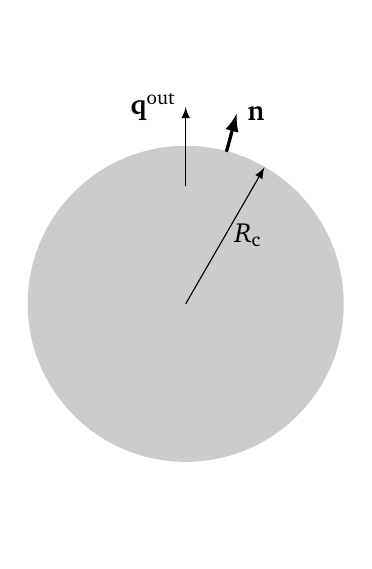
\begin{tikzpicture}
      \draw[dashed,white] (0,-3) -- (0,3.5);
      \filldraw[black!20!white] (0,0) circle [radius=2cm];
      \draw[->] (0,0) -- node[midway,right]{$R_{\mathrm{c}}$}(60:2cm);
      \draw[->] (90:1.5cm) -- (90:2.5cm) node[left]{$\mathbf{q}^{\mathrm{out}}$};
      \draw[very thick,->] (75:2cm) -- (75:2.5cm) node[right]{$\mathbf{n}$};
      \end{tikzpicture}
      \caption{Heat flow through core's surface.}
      \label{fig:flujo_nucleo}
      \end{subfigure}
~
      \begin{subfigure}[b]{0.45\textwidth}
       \centering
       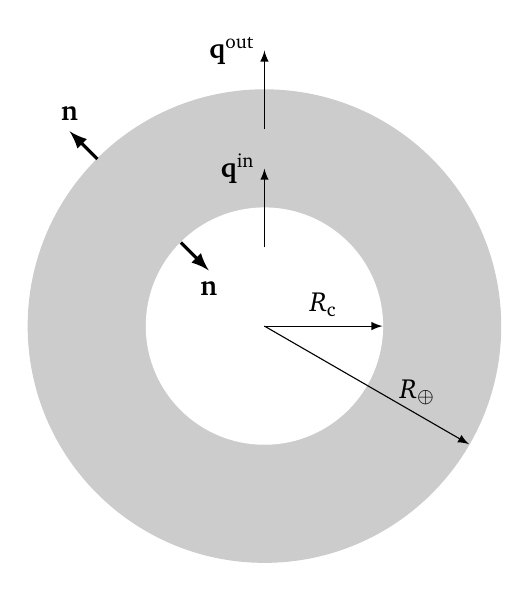
\begin{tikzpicture}
       \draw[dashed,white] (0,-3) -- (0,3.5);
       \filldraw[black!20!white] (0,0) circle [radius=3cm];
       \filldraw[white] (0,0) circle [radius=1.5cm];
       \draw[->] (0,0) -- node[midway,above]{$R_{\mathrm{c}}$}(0:1.5cm);
       \draw[->] (0,0) --  node[near end,above]{$R_{\oplus}$}(-30:3cm);
       \draw[->] (90:1cm) -- (90:2cm) node[left]{$\mathbf{q}^{\mathrm{in}}$};
       \draw[->] (90:2.5cm) -- (90:3.5cm) node[left]{$\mathbf{q}^{\mathrm{out}}$};
       \draw[very thick,->] (135:3cm) -- (135:3.5cm) node[above]{$\mathbf{n}$};
       \draw[very thick,<-] (135:1cm)node[below]{$\mathbf{n}$} -- (135:1.5cm);
      \end{tikzpicture}
      \caption{Heat flow through inner and outer surfaces of the mantle.}
      \label{fig:flujo_manto}
      \end{subfigure}
      \caption{\label{fig:Earth_interior} Schematics of the Earth's interior structure. Heat flow through the core surface (\subref{fig:flujo_nucleo}) and the inner and outer surfaces of the mantle (\subref{fig:flujo_manto}).}
\end{figure*}

Both the thermal evolution of the core and the mantle are obtained from the energy balance within each layer. That is, the time evolution of the average internal temperatures of the mantle and core are determined by the balance between the incoming and outgoing heat flux, heat sources and sinks. Among the energy sources are considered radiative decay, both in the mantle and in the core, and the aforementioned tidal interaction, which is assumed to be uniformly distributed in the mantle only. The energy sinks of the mantle are the heat that propagates by convection from the core to the surface and the heat absorbed by the material that composes the mantle at the moment of melting (latent heat).

\section{Theoretical background\label{sec:theory}}

\section{Model implementation\label{sec:model}}

\bibliographystyle{aa}
\bibliography{refs}{}

\end{document}